% Options for packages loaded elsewhere
\PassOptionsToPackage{unicode}{hyperref}
\PassOptionsToPackage{hyphens}{url}
%
\documentclass[
]{article}
\usepackage{lmodern}
\usepackage{amssymb,amsmath}
\usepackage{ifxetex,ifluatex}
\ifnum 0\ifxetex 1\fi\ifluatex 1\fi=0 % if pdftex
  \usepackage[T1]{fontenc}
  \usepackage[utf8]{inputenc}
  \usepackage{textcomp} % provide euro and other symbols
\else % if luatex or xetex
  \usepackage{unicode-math}
  \defaultfontfeatures{Scale=MatchLowercase}
  \defaultfontfeatures[\rmfamily]{Ligatures=TeX,Scale=1}
\fi
% Use upquote if available, for straight quotes in verbatim environments
\IfFileExists{upquote.sty}{\usepackage{upquote}}{}
\IfFileExists{microtype.sty}{% use microtype if available
  \usepackage[]{microtype}
  \UseMicrotypeSet[protrusion]{basicmath} % disable protrusion for tt fonts
}{}
\makeatletter
\@ifundefined{KOMAClassName}{% if non-KOMA class
  \IfFileExists{parskip.sty}{%
    \usepackage{parskip}
  }{% else
    \setlength{\parindent}{0pt}
    \setlength{\parskip}{6pt plus 2pt minus 1pt}}
}{% if KOMA class
  \KOMAoptions{parskip=half}}
\makeatother
\usepackage{xcolor}
\IfFileExists{xurl.sty}{\usepackage{xurl}}{} % add URL line breaks if available
\IfFileExists{bookmark.sty}{\usepackage{bookmark}}{\usepackage{hyperref}}
\hypersetup{
  hidelinks,
  pdfcreator={LaTeX via pandoc}}
\urlstyle{same} % disable monospaced font for URLs
\usepackage{color}
\usepackage{fancyvrb}
% decrese page margins
\usepackage{geometry}[margin=0.5cm]
\newcommand{\VerbBar}{|}
\newcommand{\VERB}{\Verb[commandchars=\\\{\}]}
\DefineVerbatimEnvironment{Highlighting}{Verbatim}{commandchars=\\\{\}}
% Add ',fontsize=\small' for more characters per line
\newenvironment{Shaded}{}{}
\newcommand{\AlertTok}[1]{\textcolor[rgb]{1.00,0.00,0.00}{\textbf{#1}}}
\newcommand{\AnnotationTok}[1]{\textcolor[rgb]{0.38,0.63,0.69}{\textbf{\textit{#1}}}}
\newcommand{\AttributeTok}[1]{\textcolor[rgb]{0.49,0.56,0.16}{#1}}
\newcommand{\BaseNTok}[1]{\textcolor[rgb]{0.25,0.63,0.44}{#1}}
\newcommand{\BuiltInTok}[1]{#1}
\newcommand{\CharTok}[1]{\textcolor[rgb]{0.25,0.44,0.63}{#1}}
\newcommand{\CommentTok}[1]{\textcolor[rgb]{0.38,0.63,0.69}{\textit{#1}}}
\newcommand{\CommentVarTok}[1]{\textcolor[rgb]{0.38,0.63,0.69}{\textbf{\textit{#1}}}}
\newcommand{\ConstantTok}[1]{\textcolor[rgb]{0.53,0.00,0.00}{#1}}
\newcommand{\ControlFlowTok}[1]{\textcolor[rgb]{0.00,0.44,0.13}{\textbf{#1}}}
\newcommand{\DataTypeTok}[1]{\textcolor[rgb]{0.56,0.13,0.00}{#1}}
\newcommand{\DecValTok}[1]{\textcolor[rgb]{0.25,0.63,0.44}{#1}}
\newcommand{\DocumentationTok}[1]{\textcolor[rgb]{0.73,0.13,0.13}{\textit{#1}}}
\newcommand{\ErrorTok}[1]{\textcolor[rgb]{1.00,0.00,0.00}{\textbf{#1}}}
\newcommand{\ExtensionTok}[1]{#1}
\newcommand{\FloatTok}[1]{\textcolor[rgb]{0.25,0.63,0.44}{#1}}
\newcommand{\FunctionTok}[1]{\textcolor[rgb]{0.02,0.16,0.49}{#1}}
\newcommand{\ImportTok}[1]{#1}
\newcommand{\InformationTok}[1]{\textcolor[rgb]{0.38,0.63,0.69}{\textbf{\textit{#1}}}}
\newcommand{\KeywordTok}[1]{\textcolor[rgb]{0.00,0.44,0.13}{\textbf{#1}}}
\newcommand{\NormalTok}[1]{#1}
\newcommand{\OperatorTok}[1]{\textcolor[rgb]{0.40,0.40,0.40}{#1}}
\newcommand{\OtherTok}[1]{\textcolor[rgb]{0.00,0.44,0.13}{#1}}
\newcommand{\PreprocessorTok}[1]{\textcolor[rgb]{0.74,0.48,0.00}{#1}}
\newcommand{\RegionMarkerTok}[1]{#1}
\newcommand{\SpecialCharTok}[1]{\textcolor[rgb]{0.25,0.44,0.63}{#1}}
\newcommand{\SpecialStringTok}[1]{\textcolor[rgb]{0.73,0.40,0.53}{#1}}
\newcommand{\StringTok}[1]{\textcolor[rgb]{0.25,0.44,0.63}{#1}}
\newcommand{\VariableTok}[1]{\textcolor[rgb]{0.10,0.09,0.49}{#1}}
\newcommand{\VerbatimStringTok}[1]{\textcolor[rgb]{0.25,0.44,0.63}{#1}}
\newcommand{\WarningTok}[1]{\textcolor[rgb]{0.38,0.63,0.69}{\textbf{\textit{#1}}}}
\usepackage{graphicx}
\makeatletter
\def\maxwidth{\ifdim\Gin@nat@width>\linewidth\linewidth\else\Gin@nat@width\fi}
\def\maxheight{\ifdim\Gin@nat@height>\textheight\textheight\else\Gin@nat@height\fi}
\makeatother
% Scale images if necessary, so that they will not overflow the page
% margins by default, and it is still possible to overwrite the defaults
% using explicit options in \includegraphics[width, height, ...]{}
\setkeys{Gin}{width=\maxwidth,height=\maxheight,keepaspectratio}
% Set default figure placement to htbp
\makeatletter
\def\fps@figure{htbp}
\makeatother
\setlength{\emergencystretch}{3em} % prevent overfull lines
\providecommand{\tightlist}{%
  \setlength{\itemsep}{0pt}\setlength{\parskip}{0pt}}
\setcounter{secnumdepth}{-\maxdimen} % remove section numbering

\author{}
\date{}

\begin{document}

\hypertarget{download-and-install-java}{%
\section{Download and install java}\label{download-and-install-java}}

\begin{figure}
\centering
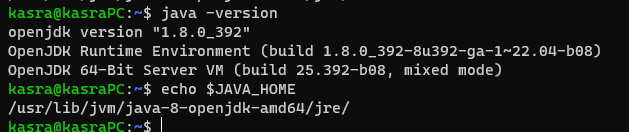
\includegraphics{image_2024-02-26_21-09-03.png}
\caption{alt text}
\end{figure}

also to set the \texttt{JAVA\_HOME} we used the following command:

\begin{Shaded}
\begin{Highlighting}[]
\BuiltInTok{export} \VariableTok{JAVA\_HOME=$(}\FunctionTok{readlink}\NormalTok{ {-}f /usr/bin/java }\KeywordTok{|} \FunctionTok{sed} \StringTok{"s:bin/java::"}\VariableTok{)}
\end{Highlighting}
\end{Shaded}

\hypertarget{download-and-install-scala}{%
\section{Download and install Scala}\label{download-and-install-scala}}

\begin{figure}
\centering
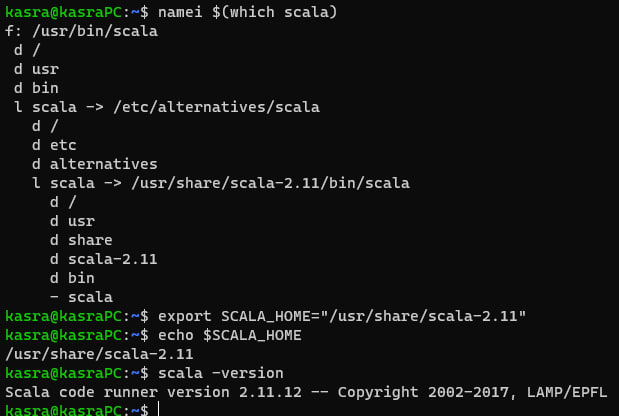
\includegraphics{image.png}
\caption{alt text}
\end{figure}

also, we could use this command to set the \texttt{SCALA\_HOME}:

\begin{Shaded}
\begin{Highlighting}[]
\BuiltInTok{export} \VariableTok{SCALA\_HOME=$(}\FunctionTok{readlink}\NormalTok{ {-}f /usr/bin/scala }\KeywordTok{|} \FunctionTok{sed} \StringTok{"s:bin/scala::"}\VariableTok{)}
\end{Highlighting}
\end{Shaded}

since \texttt{which\ scala} and \texttt{which\ scalac} works fine (they
have links in \texttt{/usr/bin}), we dont need to add the
\texttt{SCALA\_HOME} to the \texttt{PATH} but anyway, we can set it
using the following command:

\begin{Shaded}
\begin{Highlighting}[]
\BuiltInTok{export} \VariableTok{PATH=$PATH}\NormalTok{:}\VariableTok{$SCALA\_HOME}\NormalTok{/bin}
\end{Highlighting}
\end{Shaded}

\hypertarget{download-and-install-hadoop}{%
\section{Download and install
Hadoop}\label{download-and-install-hadoop}}

\begin{figure}
\centering
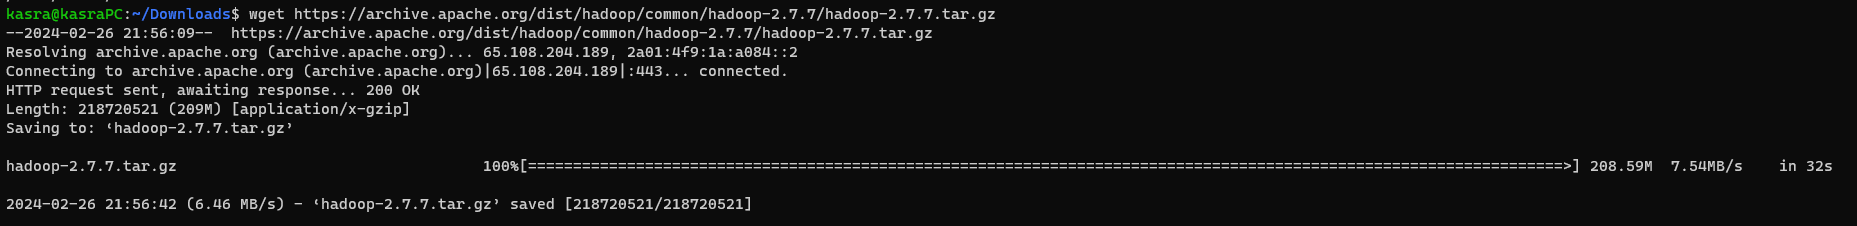
\includegraphics{image-2.png}
\caption{alt text}
\end{figure}

in the above commands, we downloaded the hadoop 2.7 from the official
website and we can extracted it to \texttt{\textasciitilde{}/.hadoop}
directory using the following command:

\begin{Shaded}
\begin{Highlighting}[]
\FunctionTok{tar}\NormalTok{ {-}xf hadoop{-}2.7.7.tar.gz}
\FunctionTok{rm}\NormalTok{ {-}rf \textasciitilde{}/.hadoop}
\FunctionTok{mkdir}\NormalTok{ \textasciitilde{}/.hadoop {-}p}
\FunctionTok{mv}\NormalTok{ hadoop{-}2.7.7/* \textasciitilde{}/.hadoop}
\FunctionTok{rmdir}\NormalTok{ hadoop{-}2.7.7}
\end{Highlighting}
\end{Shaded}

to set the \texttt{HADOOP\_HOME} and adding it to the \texttt{PATH} we
used the following commands:

\begin{Shaded}
\begin{Highlighting}[]
\BuiltInTok{export} \VariableTok{HADOOP\_HOME=}\NormalTok{\textasciitilde{}/.hadoop}
\BuiltInTok{export} \VariableTok{PATH=}\NormalTok{\textasciitilde{}/.hadoop/bin:}\VariableTok{$PATH}
\end{Highlighting}
\end{Shaded}

finally, to verify the installation:\\
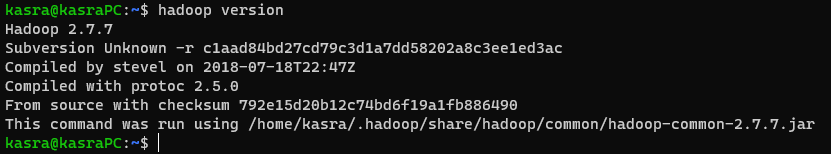
\includegraphics{image-1.png}

\hypertarget{download-and-install-spark}{%
\section{Download and install Spark}\label{download-and-install-spark}}

download the spark 3.2.1:\\
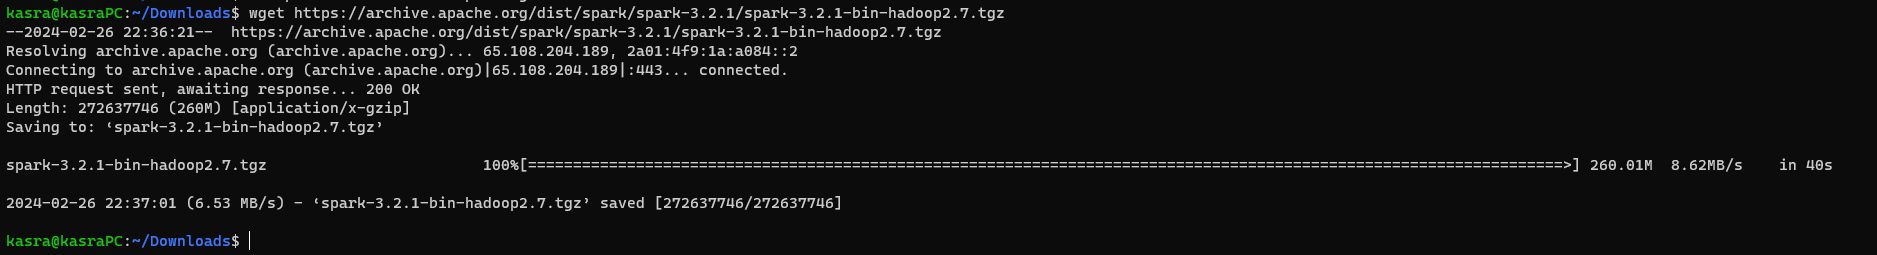
\includegraphics{image-3.png}

extract the spark to \texttt{\textasciitilde{}/.spark}:\\
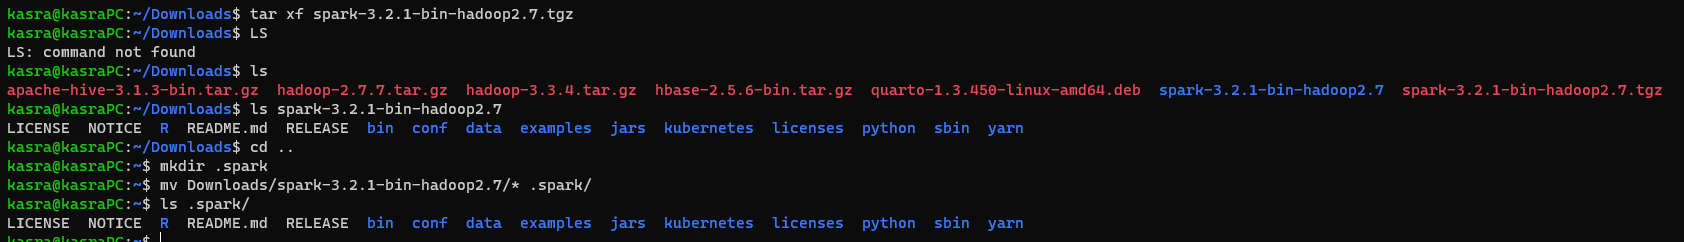
\includegraphics{image-4.png}

set the \texttt{SPARK\_HOME} and add it to the \texttt{PATH}:

\begin{Shaded}
\begin{Highlighting}[]
\BuiltInTok{export} \VariableTok{SPARK\_HOME=}\NormalTok{\textasciitilde{}/.spark}
\BuiltInTok{export} \VariableTok{PATH=}\NormalTok{\textasciitilde{}/.spark/bin:}\VariableTok{$PATH}
\end{Highlighting}
\end{Shaded}

finally, to verify the installation:\\
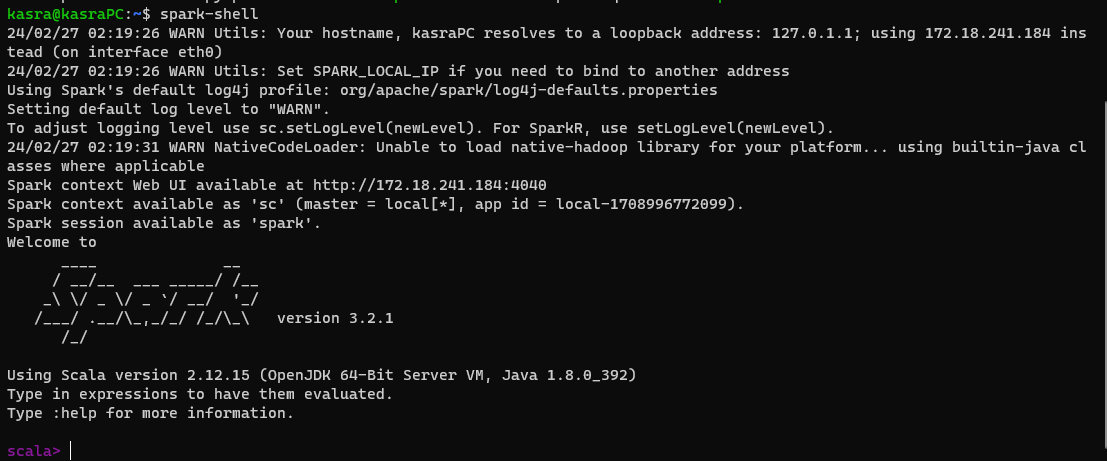
\includegraphics{image-5.png}

\hypertarget{run-the-wordcount-example-in-apache-hadoop}{%
\section{Run the WordCount example in Apache
Hadoop}\label{run-the-wordcount-example-in-apache-hadoop}}

to make a jar file using the codes, we need to compile the codes using
the following command:

\begin{Shaded}
\begin{Highlighting}[]
\ExtensionTok{javac}\NormalTok{ {-}classpath }\VariableTok{$(}\ExtensionTok{hadoop}\NormalTok{ classpath}\VariableTok{)}\NormalTok{ *.java}
\end{Highlighting}
\end{Shaded}

to verify the compliation:\\
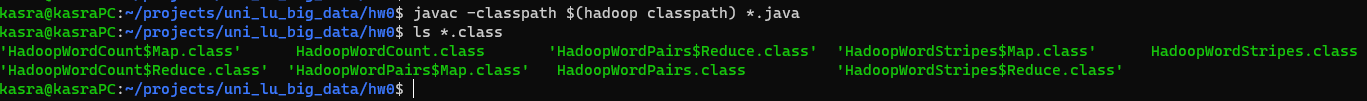
\includegraphics{image-6.png}

finally, to make a jar file:

\begin{Shaded}
\begin{Highlighting}[]
\ExtensionTok{jar}\NormalTok{ cf wc.jar *.class}
\end{Highlighting}
\end{Shaded}

in this point we can delete the \texttt{.class} files to keep the
directory clean:

\begin{Shaded}
\begin{Highlighting}[]
\FunctionTok{rm}\NormalTok{ *.class}
\end{Highlighting}
\end{Shaded}

Now we can use this command to run the \texttt{HadoopWordCount}:

\begin{Shaded}
\begin{Highlighting}[]
\ExtensionTok{hadoop}\NormalTok{ jar HadoopWordCount.jar HadoopWordCount \textasciitilde{}/data/wikipedia/enwiki{-}articles/AA/ output}
\end{Highlighting}
\end{Shaded}

to verify the output:\\
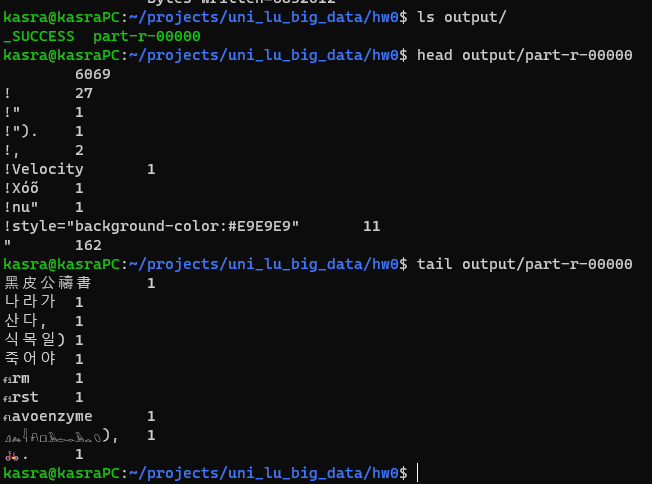
\includegraphics{image-7.png}

for the \texttt{HadoopWordPairs}:

\begin{Shaded}
\begin{Highlighting}[]
\FunctionTok{rm}\NormalTok{ {-}rf output}
\ExtensionTok{hadoop}\NormalTok{ jar HadoopWordCount.jar HadoopWordPairs \textasciitilde{}/data/wikipedia/enwiki{-}articles/AA/ output}
\end{Highlighting}
\end{Shaded}

to verify the output:\\
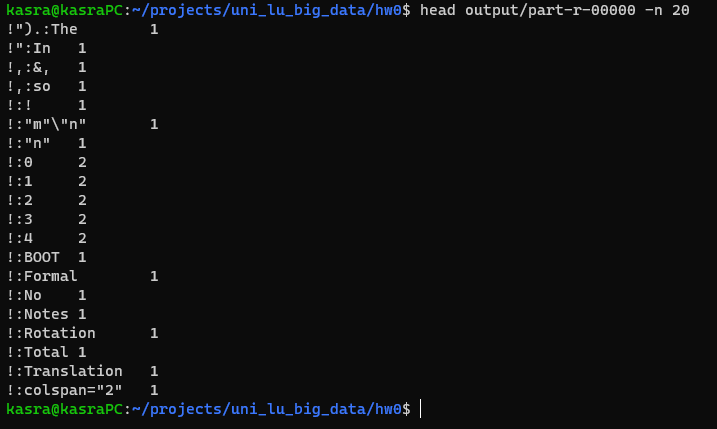
\includegraphics{image-8.png}

for the \texttt{HadoopWordStripes}:

\begin{Shaded}
\begin{Highlighting}[]
\FunctionTok{rm}\NormalTok{ {-}rf output}
\ExtensionTok{hadoop}\NormalTok{ jar HadoopWordCount.jar HadoopWordStripes \textasciitilde{}/data/wikipedia/enwiki{-}articles/AA/ output}
\end{Highlighting}
\end{Shaded}

to verify the output:\\
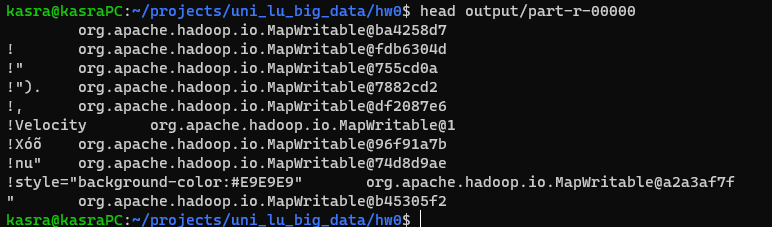
\includegraphics{image-9.png}

\hypertarget{run-the-wordcount-example-in-apache-spark}{%
\section{Run the WordCount Example in Apache
Spark}\label{run-the-wordcount-example-in-apache-spark}}

to run the \texttt{SparkWordCount} we need to install sbt using
\href{https://www.scala-sbt.org/1.x/docs/Installing-sbt-on-Linux.html}{here}
and then we need a \texttt{build.sbt} file as follows:

\begin{Shaded}
\begin{Highlighting}[]
\NormalTok{name := }\StringTok{"Simple Project"}

\NormalTok{version := }\StringTok{"1.0"}

\NormalTok{scalaVersion := }\StringTok{"2.12.18"}

\NormalTok{libraryDependencies += }\StringTok{"org.apache.spark"}\NormalTok{ \%\% }\StringTok{"spark{-}sql"}\NormalTok{ \% }\StringTok{"3.5.0"}
\end{Highlighting}
\end{Shaded}

we need to make a directory structure as follows:

\begin{verbatim}
$ find src build.*
src
src/main
src/main/scala
src/main/scala/SparkWordCount.scala
build.sbt
\end{verbatim}

and then we can use the following command to run the
\texttt{SparkWordCount}:

\begin{Shaded}
\begin{Highlighting}[]
\ExtensionTok{sbt}\NormalTok{ package}
\ExtensionTok{spark{-}submit}\NormalTok{ {-}{-}class SparkWordCount target/scala{-}2.12/simple{-}project\_2.12{-}1.0.jar \textasciitilde{}/data/wikipedia/enwiki{-}articles/AA/ output}
\end{Highlighting}
\end{Shaded}

to verify the output:\\
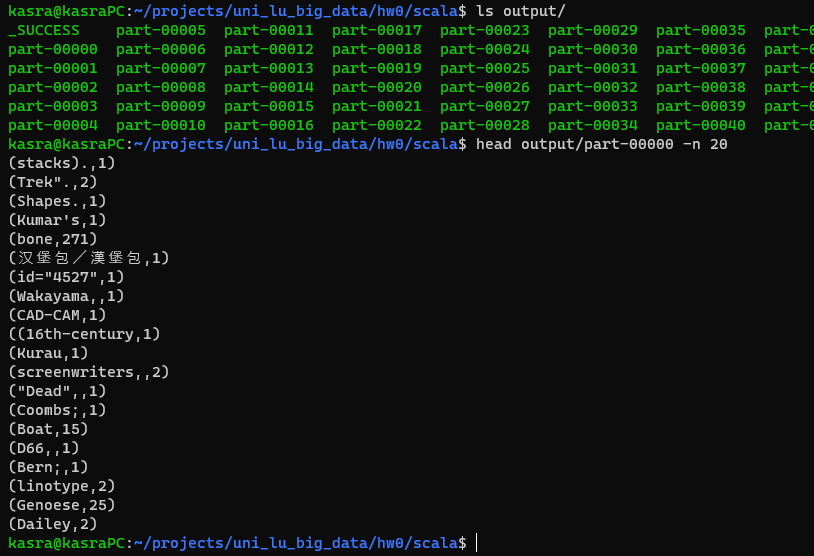
\includegraphics{image-11.png}

\end{document}
